\chapter{INTERFACE IMPLEMENTATION}
\label{chap:GUI_impl.tex}
The GUI provides user friendly and easy data navigation which will reduce debug efforts. All relevant processor execution log information and asm test details are provided to the user through a web interface. The interface uses data visualization JavaScript features to develop graphical representation of the log information. Features of the GUI are designed such that, traversing through the log information and comparison with the asm list file lines are made easy.  Major processor operations are categorized and extracted to have a clear view of processor actions.  From analysis done in Chapter 3, the following sets of features are expected to help the user and are our main design objective while implementing the interface:
\begin{itemize}

\item[-] Visualizing the processor execution flow in each thread
\item[-] Information regarding each Memory write/read, I/O write/read, Branching etc
\item[-] Interrupt and exception happening during execution
\item[-] Easy traversal to the asm instruction line.
\item[-] Register values at each instances
\item[-] Comparison of register values between two cycles
\item[-] All the cycle information provided by the cycle in execution log for detailed reference.
\end{itemize}
Once the simulation is completed and failure is reported the debug phase starts. This is where the role of GUI comes. From the vast information provided by the logs and test files, interfaces have to capture and represent relevant information to the user. The following section details the implementation and features of the proposed GUI. 

\section {INTERFACE IMPLEMENTATION}
GUI is implemented as a HTML web page. Each test case will have its one set of log files and asm list files. The interfaces implementation starts by taking these files are input.  Two programming languages are used for implementation:
\begin{itemize}
\item[-] Python Script for data extraction and correlating related information.
\item[-] JavaScript for designing the interface features and user interaction.
\end{itemize}
Figure x shows the implementation of GUI.

\addtocontents{toc}{\protect\setcounter{tocdepth}{2}}
%\figurename{} 
\begin{figure}[H]
\centering
\includegraphics[width=5.5in]{./figures/GUI_impl.eps}
\caption{GUI Implementation} 
\label{fig:GUI_impl.eps}
\end{figure}

 Major implementation steps
\begin{itemize}
\item[-] The asm list file and processor execution file informations are extracted by python script.
\item[-] A top level python program will manipulate these information are convert it to JavaScript objects. 
\item[-] JavaScript code for developing user interactive features is written.
\item[-] The top level python program will combine the data extracted and javascriot code and generate a single HTML page. 
\end{itemize}
Inputs to the implementation are Execution log file and Asm list files. To develop the GUI the user has to execute the top level python script with these two files as input argument. The script will generate an output file which is the interface web page. Major processes involved in implementation are detailed below. 


\subsection {EXTRACTING ASM FILE INFORMATION}
The test code is written in x-86 assembly language. While debugging the instructions and values in the asm file is the expected action or value.  Each cycle in processor execution log corresponds to a particular code line in asm. However the asm code written by the verification engineer is the unscheduled code without any memory address details. For cycle comparison with execution log, the asm test file is complied first.  This is done by an assembler. Figure x shows how an asm test file is converted to a list file which hold an expanded, loop unrolled, scheduled code with memory details included.  
%\figurename{} 
%\figurename{} 
\begin{figure}[H]
\centering
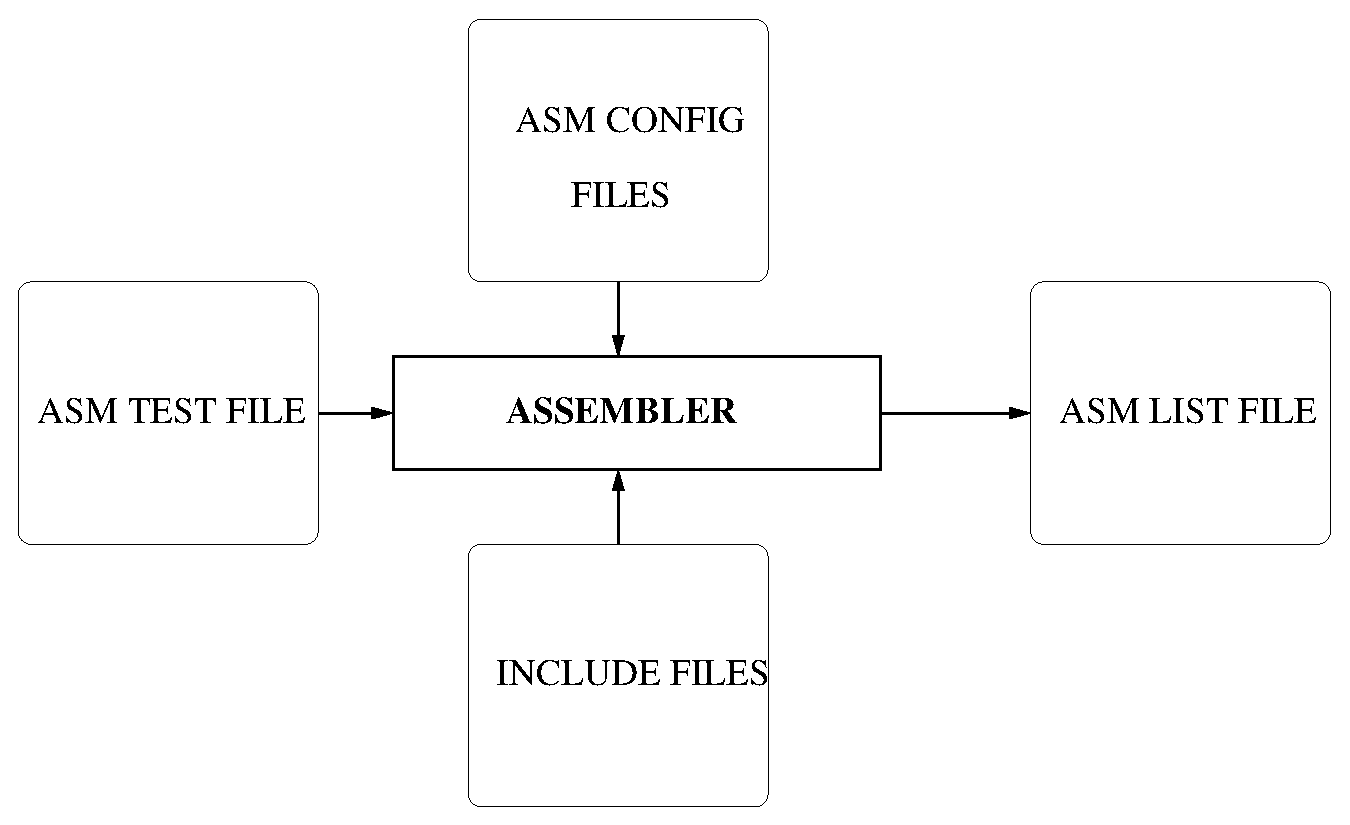
\includegraphics[width=3.5in]{./figures/asm.eps}
\caption{Assembler}
\end{figure}


A 64-bit assembler assembles asm test file, configuration file (that define the random operands, segmentation, gdt, ldt, page tables, etc,) and the include files together to generate an assembly list file [1].
\begin{figure}[H]
\centering
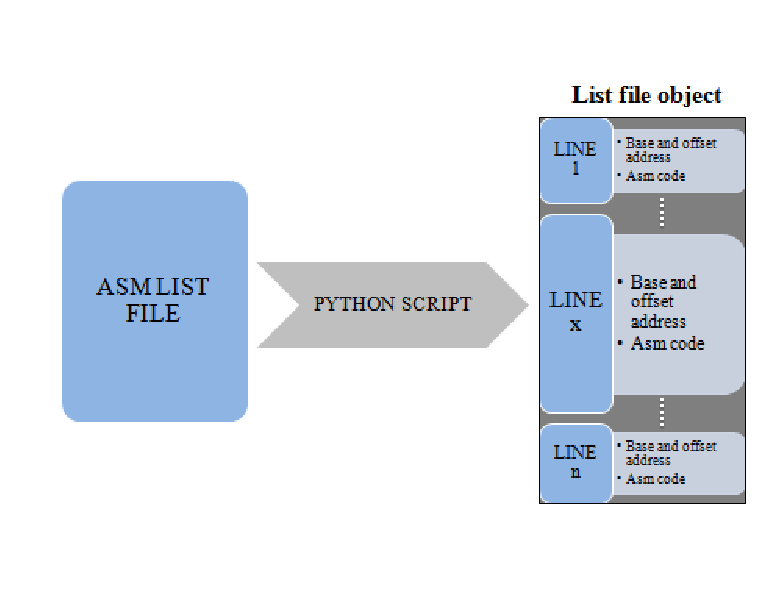
\includegraphics[width=4.5in]{./figures/list.eps}
\caption{Asm List File Extraction}
\end{figure}
List file holds details of instructions; opcodes and operand, linear address, module/register configuration details etc. For the purpose of correlating informations, a python script will extract relevant information corresponding to each instruction line in the list file.  For each line number the script will create an object which will have the following parameters.
\begin{itemize}
	\item[-] Base and offset address value
	\item[-] Instruction line number
	\item[-] The assembly code
\end{itemize}

Figure x shows how python script will read the input asm list file and generate a data structure of list objects corresponding to each line. 

\subsection {EXTRACTING EXECUTION LOG INFORMATION}
The second input to the implementation is the execution log file. As explained in previous chapters, debugging require detail traversal through this log file as it holds instruction by instruction execution details which include register states, thread details, flags information etc and other data which help in tracing out the cause of failure. 

All details given in the log file in reference to each cycle are to be extracted. The python code will extract this as well are generate a data base of log file object corresponding to each cycle of execution. These are classes with properties corresponding to major operations and register values. Each thread will have a separate handle with objects corresponding to each cycle of operation in that thread. Figure x shows how the script will read the input execution log file and generate log file objects.
Each object in the log file will have the following properties associated with it:

\begin{itemize}
 \item[-] Thread number
 \item[-]  Mode of operation
 \item[-]  Cycle number
 \item[-]  Linear address
 \item[-]  Memory write, Memory read, I/O write/read, Code read
 \item[-]  Branch target (linear address)
 \item[-]  Registers updated with new value
\end{itemize}


\subsection {Correlating asm file objects and log file objects}

Once both the input files are processed, next step is correlating the asm file object and log file object. The top level python script will combine these these to in pairs based on the address mapping. As x86 architecture follows segmented memory model along with paging, address translation is required for generating the linear/physical address [2]. For each object in the generated list file class, calculate the linear address as follows:
\\
\centerline{Linear address = Base address + Offset value}
\\
For each object in the log file class, find the corresponding list file object based on the linear address value and combine the objects.
\IncMargin{1em}
\begin{algorithm}[H]
\DontPrintSemicolon
\SetKwInOut{Input}{Input}\SetKwInOut{Output}{Output}

\Input{list file objects$\rightarrow listObj[]$, log file object$\rightarrow logObj[]$}
\Output{Test result: $pass$ or $fail$}
\BlankLine
Start: \;
For {each object $list$ in listObj}{\;
		list.address = list.Base + list.Offset\;
	}
For {each object $log$ in logObj}{\;
	set count = 0\;
	For {each object $list$ in listObj}{\;
	 \If{$log.address == list.address$}{
		Add $list.property \rightarrow log.property$\;
		count = 1;
		break loop\;
	}
	}
	\If{count == 0}{
	assert: $"no address match"$
	}
}
End \;
\caption{Memory Read-Write}
\end{algorithm}\DecMargin{1em}

\vspace{2cm}
Input: list file objects, log file objects
Start:
For each object in list file class do
	listObj.address = listObj.Base + listObj.Offset
end

For each object in log Class do
	For each object in list file class
		If logObject.address == listObj.Address
			Add listObj properties to logObject
			Break loop;
	End
	End
End
Now we have a set of objects that hold log details and are linked to corresponding asm file line. Once this stage is completed we have completed all the data extraction and next phase is building the interface.

\subsection {DEVELOP THE INTERFACE}

The final step is developing the interface. As the GUI is web based, layout design is done using HTML (Hyper Text Markup Language). However for providing interactive features to the user a much more powerful language is need along with HTML and we use JavaScript.

\emph {\bf JavaScript (JS)} is an interpreted computer programming language. It is  implemented as part of web browsers so that client-side scripts could interact with the user, control the browser, communicate asynchronously, and alter the document content that was displayed. It is a multi-paradigm language, supporting object-oriented, imperative, and functional programming styles.

In addition a style sheet language called CSS (Cascading Style Sheets) is used for describing the presentation semantics (the look and formatting) of the interface page written in HTML.

